%-----------------------------------------------------------------------------%
\chapter{IMPLEMENTASI DAN PENGUJIAN}
%-----------------------------------------------------------------------------%

%
\vspace{4.5pt}
Pada bab ini akan menjelaskan tentang pengimplementasian dan pengujian terhadap analisis sentimen yang telah dibangun berdasarkan bab-bab sebelumnya.
\section{Lingkungan Aplikasi}
Dalam aplikasi terbagi menjadi dua bagian, yaitu lingkungan implementasi perangkat keras dan perangkat lunak. Di dalam penelitian ini, perangkat keras yang digunakan adalah:
\begin{enumerate}[leftmargin=*]
	\item Processor Intel Core i3-4150 CPU 3.50GHz Dual Core
	\item RAM 8 GB.
\end{enumerate}

Spesifikasi perangkat lunak yang digunakan untuk pengembangan sistem adalah:
\begin{enumerate}[leftmargin=*]
	\item Sistem Operasi\quad\quad\quad\,: Windows 10 Enterprise 1709 64-bit.
	\item Tool Pengembangan\quad: Eclipse Java EE IDE for Web Developers.
	\item Versi\quad\quad\quad\quad\quad\quad\quad\,: Neon.3 Release (4.6.3).
\end{enumerate}

\section{Daftar \textit{Project}, \textit{Class} dan \textit{Method}}
Pada bagian ini akan dijelaskan mengenai \textit{Project}, \textit{class} dan \textit{method} yang terbentuk pada \textit{prototype} sistem Apertura dengan arsitektur microservice.
\subsection{\textit{Project} Customer}
\textit{Project Customer} berisi susunan \textit{class} pembentuk \textit{webservice customer}. Dalam project ini terdapat 4 buah \textit{package} yang berfungsi untuk memisahkan \textit{class} sesuai dengan fungsinya masing-masing. Ke empat \textit{package} ini yaitu \textit{package} controller yang berisi method-method yang dijalankan pada \textit{web service}, \textit{package} model yang berisi entitas dan tabel, \textit{package} repository yang menghubungkan entitas di \textit{package} model dengan database, dan \textit{package} service yang menginisialisasi \textit{webservice} yang akan terbentuk. Pada bagian ini akan dijelaskan mengenai \textit{class} dan \textit{method} yang digunakan pada pengembangan \textit{ webservice customer}:
\subsubsection{\textit{Package} Controller}
\textit{Package} controller berisi method API yang dapat digunakan untuk berkomunikasi dengan \textit{service} customer. \textit{Class} yang terdapat dalam \textit{package} ini adalah \textit{class} CustomerController dan CustomergroupController yang berisi 5 buah fungsi API. Di bawah ini merupakan daftar \textit{class} untuk \textit{package} controller pada \textit{webservice} customer.
\begin{table}[H]
	\small
	\centering
	\caption{Daftar {\itshape Class} pada {\itshape Package} Controller}
	\begin{adjustbox}{width=1\textwidth}
		\begin{tabular}{| p {3 cm} | p {8 cm} | p {3 cm} |}
			\hline
			{\bfseries Package} & {\bfseries Class} & {\bfseries Jenis Class} \\
			\hline
			\multirow{2}{*}{Controller} & CustomerController & {\itshape Class} \\
			& CustomergroupController & {\itshape Class} \\
			\hline
		\end{tabular}
	\end{adjustbox}
\end{table}
\begin{table}[H]
	\caption{Daftar \textit{Method} pada \textit{Class} CustomerController}
	\centering
	\small
	\begin{adjustbox}{width=1\textwidth}	
		\begin{tabular}{|p{0.4cm}|p{3.2cm}|p{1.4cm}|p{1.7cm}|p{1.55cm}|p{3cm}|}
			\hline
			\multirow{2}{*}{\textbf{No}} & \multirow{2}{*}{\textit{\textbf{Method}}} & \multicolumn{2}{c|}{\textit{\textbf{Input}}} & \multirow{2}{*}{\textit{\textbf{Output}}} & 
			\multirow{2}{*}{\textbf{Keterangan}}\\
			\cline{3-4}
			& & \textbf{Tipe} & \textbf{Variabel} & & \\
			\hline
			1 & addCustomer & void & Customer & Customer, HttpStatus & \textit{Method} ini digunakan untuk membuat \textit{object} customer yang baru melalui \textit{webservice}\\
			\hline
			2 & updateCustomer & void & Customer & HttpStatus & \textit{Method} ini digunakan untuk mengubah attribut dari \textit{object} customer yang baru melalui \textit{webservice}\\
			\hline
			3 & getCustomer & void & id & Customer, HttpStatus & \textit{Method} ini digunakan untuk mengambil satu \textit{object} customer yang baru melalui \textit{webservice}\\
			\hline
		\end{tabular}
	\end{adjustbox}
\end{table}
\begin{table}[H]
	\centering
	\small
	\begin{adjustbox}{width=1\textwidth}	
		\begin{tabular}{|p{0.4cm}|p{2.5cm}|p{1cm}|p{1.1cm}|p{3.4cm}|p{3cm}|}
			\hline
			4 & getAllCustomer & void & - & $<$List$<$Customer$>$$>$, HttpStatus & \textit{Method} ini digunakan untuk mengambil semua \textit{list} \textit{object} customer yang baru melalui \textit{webservice}\\
			\hline
			5 & deleteCustomer & void & id &HttpStatus & \textit{Method} ini digunakan untuk menghapus satu \textit{object} customer yang baru melalui \textit{webservice}\\
			\hline
		\end{tabular}
	\end{adjustbox}
\end{table}
\begin{table}[H]
	\caption{Daftar \textit{Method} pada \textit{Class} CustomergroupController}
	\centering
	\small
	\begin{adjustbox}{width=1\textwidth}	
		\begin{tabular}{|p{0.4cm}|p{3.5cm}|p{1.4cm}|p{1.7cm}|p{1.55cm}|p{3cm}|}
			\hline
			\multirow{2}{*}{\textbf{No}} & \multirow{2}{*}{\textit{\textbf{Method}}} & \multicolumn{2}{c|}{\textit{\textbf{Input}}} & \multirow{2}{*}{\textit{\textbf{Output}}} & 
			\multirow{2}{*}{\textbf{Keterangan}}\\
			\cline{3-4}
			& & \textbf{Tipe} & \textbf{Variabel} & & \\
			\hline
			1 & addCustomerGroup & Customer & customer & customer, HttpStatus & \textit{Method} ini digunakan untuk membuat \textit{object} CustomerGroup yang baru melalui \textit{webservice}\\
			\hline
			2 & updateCustomerGroup & Customer & customer & HttpStatus & \textit{Method} ini digunakan untuk mengubah attribut dari \textit{object} CustomerGroup yang baru melalui \textit{webservice}\\
			\hline
			3 & getCustomerGroup & Customer & customer & customer, HttpStatus & \textit{Method} ini digunakan untuk mengambil satu \textit{object} CustomerGroup yang baru melalui \textit{webservice}\\
			\hline
			4 & getAllCustomerGroup & Customer & customer & customer, HttpStatus & \textit{Method} ini digunakan untuk mengambil semua \textit{list} \textit{object} CustomerGroup yang baru melalui \textit{webservice}\\
			\hline
		\end{tabular}
	\end{adjustbox}
\end{table}
\begin{table}[H]
	\centering
	\small
	\begin{adjustbox}{width=1\textwidth}	
		\begin{tabular}{|p{0.4cm}|p{3.5cm}|p{1.4cm}|p{1.7cm}|p{1.55cm}|p{3cm}|}
			\hline
			5 & deleteCustomerGroup & Customer & customer & customer, HttpStatus & \textit{Method} ini digunakan untuk menghapus satu \textit{object} CustomerGroup yang baru melalui \textit{webservice}\\
			\hline
		\end{tabular}
	\end{adjustbox}
\end{table}
\subsubsection{\textit{Package} Model Customer}
\textit{Package} customer model berisi entitas-entitas penyusun dari \textit{service} customer. Berikut ini merupakan daftar \textit{class} untuk \textit{package} model.
\begin{table}[H]
	\small
	\centering
	\caption{Daftar {\itshape Class} pada {\itshape Package} model}
	\begin{adjustbox}{width=1\textwidth}
		\begin{tabular}{| p {3 cm} | p {8 cm} | p {3 cm} |}
			\hline
			{\bfseries Package} & {\bfseries Class} & {\bfseries Jenis Class} \\
			\hline
			\multirow{13}{*}{Model} & Regency & {\itshape Class} \\
			& AddressType & {\itshape Class} \\
			& Contact & {\itshape Class} \\
			& ContactAddress & {\itshape Class} \\
			& ContactEducation & {\itshape Class} \\
			& Country & {\itshape Class} \\
			& Customer & {\itshape Class} \\
			& Customergroup & {\itshape Class} \\
			& HealthConsumer & {\itshape Class} \\
			& Insurance & {\itshape Class} \\
			& InsuranceBridgeConf & {\itshape Class} \\
			& Profession & {\itshape Class} \\
			& Province & {\itshape Class} \\
			\hline
		\end{tabular}
	\end{adjustbox}
\end{table}
\begin{table}[H]
	\caption{Daftar attribut pada \textit{Class} Customer}
	\centering
	\small
	\begin{adjustbox}{width=1\textwidth}	
		\begin{tabular}{|p{4cm} p{2.1cm} p{3cm} p{3.1cm}|}
			\hline
			\multicolumn{2}{|l}{\textbf{Variabel:}}&\multicolumn{2}{l|}{\textbf{Variabel:}}\\
			boolean&cust\_no&Date&registrationdate\\
			boolean&active&int&idPriceLevel\\
			double&creditlimit&double&disc\\
			Customergroup&customergroup&&\\
			\hline
		\end{tabular}
	\end{adjustbox}
\end{table}

\begin{table}[H]
	\caption{Daftar attribut pada \textit{Class} Customergroup}
	\centering
	\small
	\begin{adjustbox}{width=1\textwidth}	
		\begin{tabular}{|p{4cm} p{2.1cm} p{3cm} p{3.1cm}|}
			\hline
			\multicolumn{2}{|l}{\textbf{Variabel:}}&\multicolumn{2}{l|}{}\\
			long&systemid&&\\
			String&groupname&&\\
			String&memo&&\\
			\hline
		\end{tabular}
	\end{adjustbox}
\end{table}

\begin{table}[H]
	\caption{Daftar attribut pada \textit{Class} Contact}
	\centering
	\small
	\begin{adjustbox}{width=1\textwidth}	
		\begin{tabular}{|p{2cm} p{2.1cm} p{5cm} p{3.1cm}|}
			\hline
			\multicolumn{2}{|l}{\textbf{Variabel:}}&\multicolumn{2}{l|}{\textbf{Variabel:}}\\
			long&systemid&String&initial\\
			String&lastname&int&amountofchildren\\
			int&maritalstatus&List$<$ContactAddress$>$&arrAddress\\
			String&middlename&Collection$<$ContactEducation$>$&arrEdu\\
			Date&birthday&String&notes\\
			String&birthplace&String&officeext\\
			String&bloodtype&String&passportid\\
			double&bodyheight&byte[]&photo\\
			double&bodyweight&String&prefixtitle\\
			String&citizenid&String&sms\\
			String&citizentype&String&suffixtitle\\
			Country&citizenship&Date&sys\_createdate\\
			String&email&String&sys\_creator\\
			String&firstname&Date&sys\_lastupdate\\
			int&gender&String&sys\_lastupdater\\
			String&homephone&String&taxid\\
			String&messaging&String&web\\
			\hline
		\end{tabular}
	\end{adjustbox}
\end{table}
\begin{table}[H]
	\caption{Daftar attribut pada \textit{Class} Contact Address}
	\centering
	\small
	\begin{adjustbox}{width=1\textwidth}	
		\begin{tabular}{|p{4cm} p{2.1cm} p{3cm} p{3.1cm}|}
			\hline
			\multicolumn{2}{|l}{\textbf{Variabel:}}&\multicolumn{2}{l|}{\textbf{Variabel:}}\\
			Long&systemid&String&postcode\\
			AddressType&addresstype&Regency&regency\\
			String&street&boolean&asbillingaddress\\
			String&fax&Date&sys\_createdate\\
			Contact&owner&String&sys\_creator\\
			String&phone&Date&sys\_lastupdate\\
			String&sys\_lastupdater&&\\
			\hline
		\end{tabular}
	\end{adjustbox}
\end{table}
\begin{table}[H]
	\caption{Daftar attribut pada \textit{Class} Address Type}
	\centering
	\small
	\begin{adjustbox}{width=1\textwidth}	
		\begin{tabular}{|p{4cm} p{2.1cm} p{3cm} p{3.1cm}|}
			\hline
			\multicolumn{2}{|l}{\textbf{Variabel:}}&\multicolumn{2}{l|}{\textbf{}}\\
			Integer&systemid&&\\
			String&memo&&\\
			String&typename&&\\
			\hline
		\end{tabular}
	\end{adjustbox}
\end{table}
\begin{table}[H]
	\caption{Daftar attribut pada \textit{Class} Contact Education}
	\centering
	\small
	\begin{adjustbox}{width=1\textwidth}	
		\begin{tabular}{|p{3cm} p{3.1cm} p{3cm} p{3.1cm}|}
			\hline
			\multicolumn{2}{|l}{\textbf{Variabel:}}&\multicolumn{2}{l|}{\textbf{\textbf{Variabel:}}}\\
			Date&finishrolling&Contact&owner\\
			String&gpa&String&sponsors\\
			int&grade&Date&startrolling\\
			String&institutionaladdress&Date&sys\_createdate\\
			String&institutionname&int&sys\_creator\\
			String&major&Date&sys\_lastupdate\\
			String&notes&int&sys\_lastupdater\\
			\hline
		\end{tabular}
	\end{adjustbox}
\end{table}
\begin{table}[H]
	\caption{Daftar attribut pada \textit{Class} Country}
	\centering
	\small
	\begin{adjustbox}{width=1\textwidth}	
		\begin{tabular}{|p{4cm} p{2.1cm} p{3cm} p{3.1cm}|}
			\hline
			\multicolumn{2}{|l}{\textbf{Variabel:}}&\multicolumn{2}{l|}{\textbf{}}\\
			Long&systemid&&\\
			String&name&&\\
			\hline
		\end{tabular}
	\end{adjustbox}
\end{table}
\begin{table}[H]
	\caption{Daftar attribut pada \textit{Class} HealthConsumer}
	\centering
	\small
	\begin{adjustbox}{width=1\textwidth}	
		\begin{tabular}{|p{4cm} p{2.1cm} p{3cm} p{3.1cm}|}
			\hline
			\multicolumn{2}{|l}{\textbf{Variabel:}}&\multicolumn{2}{l|}{\textbf{}}\\
			String&regis\_no&&\\
			Profession&id\_prof&&\\
			Insurance&insurance&&\\
			String&insurance\_type&&\\
			String&insurance\_no&&\\
			String&insurance\_prg&&\\
			\hline
		\end{tabular}
	\end{adjustbox}
\end{table}
\begin{table}[H]
	\caption{Daftar attribut pada \textit{Class} Insurance}
	\centering
	\small
	\begin{adjustbox}{width=1\textwidth}	
		\begin{tabular}{|p{5cm} p{3.1cm} p{2cm} p{2.1cm}|}
			\hline
			\multicolumn{2}{|l}{\textbf{Variabel:}}&\multicolumn{2}{l|}{\textbf{}}\\
			List$<$InsuranceBridgeConf$>$&insuranceBrigdeConfList&&\\
			int&systemid&&\\
			String&insurance&&\\
			String&memo&&\\
			boolean&active&&\\
			boolean&sysbuiltin&&\\
			\hline
		\end{tabular}
	\end{adjustbox}
\end{table}
\begin{table}[H]
	\caption{Daftar attribut pada \textit{Class} InsuranceBridgeConf}
	\centering
	\small
	\begin{adjustbox}{width=1\textwidth}	
		\begin{tabular}{|p{5cm} p{3.1cm} p{2cm} p{2.1cm}|}
			\hline
			\multicolumn{2}{|l}{\textbf{Variabel:}}&\multicolumn{2}{l|}{\textbf{}}\\
			Long&systemid&&\\
			String&field&&\\
			String&def\_val&&\\
			String&memo&&\\
			\hline
		\end{tabular}
	\end{adjustbox}
\end{table}
\begin{table}[H]
	\caption{Daftar attribut pada \textit{Class} Profession}
	\centering
	\small
	\begin{adjustbox}{width=1\textwidth}	
		\begin{tabular}{|p{5cm} p{3.1cm} p{2cm} p{2.1cm}|}
			\hline
			\multicolumn{2}{|l}{\textbf{Variabel:}}&\multicolumn{2}{l|}{\textbf{}}\\
			Integer&systemid&&\\
			String&profname&&\\
			String&memo&&\\
			Calendar&sys\_createdate&&\\
			Calendar&last\_createdate&&\\
			\hline
		\end{tabular}
	\end{adjustbox}
\end{table}
\begin{table}[H]
	\caption{Daftar attribut pada \textit{Class} Province}
	\centering
	\small
	\begin{adjustbox}{width=1\textwidth}	
		\begin{tabular}{|p{5cm} p{3.1cm} p{2cm} p{2.1cm}|}
			\hline
			\multicolumn{2}{|l}{\textbf{Variabel:}}&\multicolumn{2}{l|}{\textbf{}}\\
			Long&systemid&&\\
			Country&countryCode&&\\
			String&name&&\\
			Set$<$Regency$>$&regencySet&&\\
			\hline
		\end{tabular}
	\end{adjustbox}
\end{table}
\begin{table}[H]
	\caption{Daftar attribut pada \textit{Class} Regency}
	\centering
	\small
	\begin{adjustbox}{width=1\textwidth}	
		\begin{tabular}{|p{5cm} p{3.1cm} p{2cm} p{2.1cm}|}
			\hline
			\multicolumn{2}{|l}{\textbf{Variabel:}}&\multicolumn{2}{l|}{\textbf{}}\\
			Long&systemid&&\\
			Province&provId&&\\
			String&name&&\\
			\hline
		\end{tabular}
	\end{adjustbox}
\end{table}
\subsubsection{\textit{Package} Repository}
\textit{Package} repository berisi \textit{class-class} yang menjadi representasi model dari tabel-tabel yang berada pada basis data. Berikut ini merupakan \textit{class-class} yang terdapat pada \textit{package} repository.
\begin{table}[H]
	\small
	\centering
	\caption{Daftar {\itshape Class} pada {\itshape Package} repository}
	\begin{adjustbox}{width=1\textwidth}
		\begin{tabular}{| p {3 cm} | p {8 cm} | p {3 cm} |}
			\hline
			{\bfseries Package} & {\bfseries Class} & {\bfseries Jenis Class} \\
			\hline
			\multirow{2}{*}{repository} & CustomerRepository & {\itshape Interface} \\
			& CustomergroupRepository & {\itshape Interface} \\
			\hline
		\end{tabular}
	\end{adjustbox}
\end{table}
\subsubsection{\textit{Package} Service}
\textit{Package} service berisi \textit{class-class} yang menginisialisasi \textit{web service} customer yang akan terbentuk dan digunakan pada \textit{package} controller. Berikut ini merupakan \textit{class-class} yang terdapat pada \textit{package} service.
\begin{table}[H]
	\small
	\centering
	\caption{Daftar {\itshape Class} pada {\itshape Package} serviec}
	\begin{adjustbox}{width=1\textwidth}
		\begin{tabular}{| p {3 cm} | p {8 cm} | p {3 cm} |}
			\hline
			{\bfseries Package} & {\bfseries Class} & {\bfseries Jenis Class} \\
			\hline
			\multirow{5}{*}{service} & CRUDService & {\itshape Interface} \\
			& CustomergroupService & {\itshape Interface} \\
			& CustomerService & {\itshape Interface} \\
			& DefaultCustomergroupService & {\itshape Class} \\
			& DefaultCustomerService & {\itshape Class} \\
			\hline
		\end{tabular}
	\end{adjustbox}
\end{table}
\subsection{\textit{Project} \textit{Human Resource}}
\textit{Project Human Resource} berisi susunan \textit{class} pembentuk \textit{webservice Human Resource}. Dalam project ini terdapat 4 buah \textit{package} yang berfungsi untuk memisahkan \textit{class} sesuai dengan fungsinya masing-masing. Ke empat \textit{package} ini yaitu \textit{package} controller yang berisi method-method yang dijalankan pada \textit{web service}, \textit{package} model yang berisi entitas dan tabel, \textit{package} repository yang menghubungkan entitas di \textit{package} model dengan database, dan \textit{package} service yang menginisialisasi \textit{webserviec} yang akan terbentuk. Pada bagian ini akan dijelaskan mengenai \textit{class} dan \textit{method} yang digunakan pada pengembangan \textit{ webservice customer}:
\subsubsection{\textit{Package} Controller}
\textit{Package} controller berisi method API yang dapat digunakan untuk berkomunikasi dengan \textit{service} Human Resource. \textit{Class} yang terdapat dalam \textit{package} ini adalah \textit{class} EmployeeController dan JobSpecialityController yang berisi 5 buah fungsi API. Di bawah ini merupakan daftar \textit{class} untuk \textit{package} controller pada \textit{webservice} \textit{Human Resource}.
\begin{table}[H]
	\small
	\centering
	\caption{Daftar {\itshape Class} pada {\itshape Package} Controller}
	\begin{adjustbox}{width=1\textwidth}
		\begin{tabular}{| p {3 cm} | p {8 cm} | p {3 cm} |}
			\hline
			{\bfseries Package} & {\bfseries Class} & {\bfseries Jenis Class} \\
			\hline
			\multirow{2}{*}{Controller} & EmployeeController & {\itshape Class} \\
			& JobspecialityController & {\itshape Class} \\
			\hline
		\end{tabular}
	\end{adjustbox}
\end{table}
\begin{table}[H]
	\caption{Daftar \textit{Method} pada \textit{Class} EmployeeController}
	\centering
	\small
	\begin{adjustbox}{width=1\textwidth}	
		\begin{tabular}{|p{0.4cm}|p{2.5cm}|p{0.9cm}|p{1.5cm}|p{3.4cm}|p{2.5cm}|}
			\hline
			\multirow{2}{*}{\textbf{No}} & \multirow{2}{*}{\textit{\textbf{Method}}} & \multicolumn{2}{c|}{\textit{\textbf{Input}}} & \multirow{2}{*}{\textit{\textbf{Output}}} & 
			\multirow{2}{*}{\textbf{Keterangan}}\\
			\cline{3-4}
			& & \textbf{Tipe} & \textbf{Variabel} & & \\
			\hline
			1 & addEmployee & void & Employee & Employee, HttpStatus & \textit{Method} ini digunakan untuk membuat \textit{object} employee yang baru melalui \textit{webservice}\\
			\hline
			2 & updateEmployee & void & Employee & HttpStatus & \textit{Method} ini digunakan untuk mengubah attribut dari \textit{object} employee yang baru melalui \textit{webservice}\\
			\hline
			3 & getEmployee & void & id & Employee, HttpStatus & \textit{Method} ini digunakan untuk mengambil satu \textit{object} employee yang baru melalui \textit{webservice}\\
			\hline
			4 & getAllEmployees & void & - & $<$List$<$Employee$>$$>$, HttpStatus & \textit{Method} ini digunakan untuk mengambil semua \textit{list} \textit{object} employee yang baru melalui \textit{webservice}\\
			\hline
		\end{tabular}
	\end{adjustbox}
\end{table}
\begin{table}[H]
	\centering
	\small
	\begin{adjustbox}{width=1\textwidth}	
		\begin{tabular}{|p{0.4cm}|p{2.5cm}|p{0.9cm}|p{1.5cm}|p{3.4cm}|p{2.5cm}|}
			\hline
			5 & deleteEmployee & void & id & HttpStatus & \textit{Method} ini digunakan untuk menghapus satu \textit{object} employee yang baru melalui \textit{webservice}\\
			\hline
		\end{tabular}
	\end{adjustbox}
\end{table}
\begin{table}[H]
	\caption{Daftar \textit{Method} pada \textit{Class} JobspecialityController}
	\centering
	\small
	\begin{adjustbox}{width=1\textwidth}	
		\begin{tabular}{|p{0.4cm}|p{3.2cm}|p{0.8cm}|p{1.9cm}|p{2.85cm}|p{2.4cm}|}
			\hline
			\multirow{2}{*}{\textbf{No}} & \multirow{2}{*}{\textit{\textbf{Method}}} & \multicolumn{2}{c|}{\textit{\textbf{Input}}} & \multirow{2}{*}{\textit{\textbf{Output}}} & 
			\multirow{2}{*}{\textbf{Keterangan}}\\
			\cline{3-4}
			& & \textbf{Tipe} & \textbf{Variabel} & & \\
			\hline
			1 & addJobSpeciality & void & Jobspeciality & Jobspeciality, HttpStatus & \textit{Method} ini digunakan untuk membuat \textit{object} Jobspeciality yang baru melalui \textit{webservice}\\
			\hline
			2 & updateJobSpeciality & void & Jobspeciality & HttpStatus & \textit{Method} ini digunakan untuk mengubah attribut dari \textit{object} Jobspeciality yang baru melalui \textit{webservice}\\
			\hline
			3 & getJobSpeciality & void & id & Jobspeciality, HttpStatus & \textit{Method} ini digunakan untuk mengambil satu \textit{object} Jobspeciality yang baru melalui \textit{webservice}\\
			\hline
		\end{tabular}
	\end{adjustbox}
\end{table}
\begin{table}[H]
	\centering
	\small
	\begin{adjustbox}{width=1\textwidth}	
		\begin{tabular}{|p{0.4cm}|p{3.2cm}|p{1.cm}|p{1.7cm}|p{2.75cm}|p{2.5cm}|}
			\hline
			4 & getAllJobsSpeciality & void & - & $<$List
			$<$Jobspeciality$>$$>$, HttpStatus & \textit{Method} ini digunakan untuk mengambil semua \textit{list} \textit{object} Jobspeciality yang baru melalui \textit{webservice}\\
			\hline
			5 & deleteJobSpeciality & void & id & Jobspeciality, HttpStatus & \textit{Method} ini digunakan untuk menghapus satu \textit{object} CustomerGroup yang baru melalui \textit{webservice}\\
			\hline
		\end{tabular}
	\end{adjustbox}
\end{table}
\subsubsection{\textit{Package} Model Human Resource}
\textit{Package} Human Resource model berisi entitas-entitas penyusun dari \textit{service} Human Resource. Berikut ini merupakan daftar \textit{class} untuk \textit{package} model.
\begin{table}[H]
	\small
	\centering
	\caption{Daftar {\itshape Class} pada {\itshape Package} model}
	\begin{adjustbox}{width=1\textwidth}
		\begin{tabular}{| p {3 cm} | p {8 cm} | p {3 cm} |}
			\hline
			{\bfseries Package} & {\bfseries Class} & {\bfseries Jenis Class} \\
			\hline
			\multirow{12}{*}{Model} & Regency & {\itshape Class} \\
			& AddressType & {\itshape Class} \\
			& Contact & {\itshape Class} \\
			& ContactAddress & {\itshape Class} \\
			& ContactEducation & {\itshape Class} \\
			& Country & {\itshape Class} \\
			& Department & {\itshape Class} \\
			& Employee & {\itshape Class} \\
			& Employment & {\itshape Class} \\
			& Jobspeciality & {\itshape Class} \\
			& Province & {\itshape Class} \\
			& RoleInDept & {\itshape Class} \\
			\hline
		\end{tabular}
	\end{adjustbox}
\end{table}
\begin{table}[H]
	\caption{Daftar attribut pada \textit{Class} Employment}
	\centering
	\small
	\begin{adjustbox}{width=1\textwidth}	
		\begin{tabular}{|p{4cm} p{2.1cm} p{3cm} p{3.1cm}|}
			\hline
			\multicolumn{2}{|l}{\textbf{Variabel:}}&\multicolumn{2}{l|}{\textbf{Variabel:}}\\
			Long&systemid&Employee&employee\\
			String&ein&Date&hiredate\\
			BigInteger&basesalary&RoleInDept&roleIndept\\
			Integer&contracttype&String& sourceinstitution\\
			int&sourcetype&Date& createdate\\
			Date&lastupdate&Date& terminatedate\\
			\hline
		\end{tabular}
	\end{adjustbox}
\end{table}
\begin{table}[H]
	\caption{Daftar attribut pada \textit{Class} Employee}
	\centering
	\small
	\begin{adjustbox}{width=1\textwidth}	
		\begin{tabular}{|p{4cm} p{2.1cm} p{3cm} p{3.1cm}|}
			\hline
			\multicolumn{2}{|l}{\textbf{Variabel:}}&\multicolumn{2}{l|}{}\\
			String&m\_ein&&\\
			Jobspeciality&jobspeciality&&\\
			Collection$<$Employment$>$&employmentCollection&&\\
			\hline
		\end{tabular}
	\end{adjustbox}
\end{table}
\begin{table}[H]
	\caption{Daftar attribut pada \textit{Class} Departement}
	\centering
	\small
	\begin{adjustbox}{width=1\textwidth}	
		\begin{tabular}{|p{4cm} p{2.1cm} p{3cm} p{3.1cm}|}
			\hline
			\multicolumn{2}{|l}{\textbf{Variabel:}}&\multicolumn{2}{l|}{\textbf{}}\\
			int&systemid&&\\
			String&deptname&&\\
			String&memo&&\\
			Collection$<$RoleInDept$>$&roles&&\\
			Date&createdate&&\\
			Date&lastupdate&&\\
			\hline
		\end{tabular}
	\end{adjustbox}
\end{table}
\begin{table}[H]
	\caption{Daftar attribut pada \textit{Class} Contact}
	\centering
	\small
	\begin{adjustbox}{width=1\textwidth}	
		\begin{tabular}{|p{2cm} p{2.1cm} p{5cm} p{3.1cm}|}
			\hline
			\multicolumn{2}{|l}{\textbf{Variabel:}}&\multicolumn{2}{l|}{\textbf{Variabel:}}\\
			long&systemid&String&initial\\
			String&lastname&int&amountofchildren\\
			int&maritalstatus&List$<$ContactAddress$>$&arrAddress\\
			String&middlename&Collection$<$ContactEducation$>$&arrEdu\\
			Date&birthday&String&notes\\
			String&birthplace&String&officeext\\
			String&bloodtype&String&passportid\\
			double&bodyheight&byte[]&photo\\
			double&bodyweight&String&prefixtitle\\
			String&citizenid&String&sms\\
			String&citizentype&String&suffixtitle\\
			Country&citizenship&Date&sys\_createdate\\
			String&email&String&sys\_creator\\
			String&firstname&Date&sys\_lastupdate\\
			int&gender&String&sys\_lastupdater\\
			String&homephone&String&taxid\\
			String&messaging&String&web\\
			\hline
		\end{tabular}
	\end{adjustbox}
\end{table}
\begin{table}[H]
	\caption{Daftar attribut pada \textit{Class} ContactAddress}
	\centering
	\small
	\begin{adjustbox}{width=1\textwidth}	
		\begin{tabular}{|p{4cm} p{2.1cm} p{3cm} p{3.1cm}|}
			\hline
			\multicolumn{2}{|l}{\textbf{Variabel:}}&\multicolumn{2}{l|}{\textbf{Variabel:}}\\
			Long&systemid&String&postcode\\
			AddressType&addresstype&Regency&regency\\
			String&street&boolean&asbillingaddress\\
			String&fax&Date&sys\_createdate\\
			Contact&owner&String&sys\_creator\\
			String&phone&Date&sys\_lastupdate\\
			String&sys\_lastupdater&&\\
			\hline
		\end{tabular}
	\end{adjustbox}
\end{table}
\begin{table}[H]
	\caption{Daftar attribut pada \textit{Class} AddressType}
	\centering
	\small
	\begin{adjustbox}{width=1\textwidth}	
		\begin{tabular}{|p{4cm} p{2.1cm} p{3cm} p{3.1cm}|}
			\hline
			\multicolumn{2}{|l}{\textbf{Variabel:}}&\multicolumn{2}{l|}{\textbf{}}\\
			Integer&systemid&&\\
			String&memo&&\\
			String&typename&&\\
			\hline
		\end{tabular}
	\end{adjustbox}
\end{table}
\begin{table}[H]
	\caption{Daftar attribut pada \textit{Class} ContactEducation}
	\centering
	\small
	\begin{adjustbox}{width=1\textwidth}	
		\begin{tabular}{|p{3cm} p{3.1cm} p{3cm} p{3.1cm}|}
			\hline
			\multicolumn{2}{|l}{\textbf{Variabel:}}&\multicolumn{2}{l|}{\textbf{\textbf{Variabel:}}}\\
			Date&finishrolling&Contact&owner\\
			String&gpa&String&sponsors\\
			int&grade&Date&startrolling\\
			String&institutionaladdress&Date&sys\_createdate\\
			String&institutionname&int&sys\_creator\\
			String&major&Date&sys\_lastupdate\\
			String&notes&int&sys\_lastupdater\\
			\hline
		\end{tabular}
	\end{adjustbox}
\end{table}
\begin{table}[H]
	\caption{Daftar attribut pada \textit{Class} Country}
	\centering
	\small
	\begin{adjustbox}{width=1\textwidth}	
		\begin{tabular}{|p{4cm} p{2.1cm} p{3cm} p{3.1cm}|}
			\hline
			\multicolumn{2}{|l}{\textbf{Variabel:}}&\multicolumn{2}{l|}{\textbf{}}\\
			Long&systemid&&\\
			String&name&&\\
			\hline
		\end{tabular}
	\end{adjustbox}
\end{table}
\begin{table}[H]
	\caption{Daftar attribut pada \textit{Class} Jobspeciality}
	\centering
	\small
	\begin{adjustbox}{width=1\textwidth}	
		\begin{tabular}{|p{5cm} p{3.1cm} p{2cm} p{2.1cm}|}
			\hline
			\multicolumn{2}{|l}{\textbf{Variabel:}}&\multicolumn{2}{l|}{\textbf{}}\\
			Long&systemid&&\\
			String&specialityName&&\\
			String&memo&&\\
			\hline
		\end{tabular}
	\end{adjustbox}
\end{table}
\begin{table}[H]
	\caption{Daftar attribut pada \textit{Class} RoleInDept}
	\centering
	\small
	\begin{adjustbox}{width=1\textwidth}	
		\begin{tabular}{|p{5cm} p{3.1cm} p{2cm} p{2.1cm}|}
			\hline
			\multicolumn{2}{|l}{\textbf{Variabel:}}&\multicolumn{2}{l|}{\textbf{}}\\
			int&systemid&&\\
			Department&department&&\\
			String&rolename&&\\
			String&abbreviation&&\\
			RoleInDept&parentRole&&\\
			String&memo&&\\
			\hline
		\end{tabular}
	\end{adjustbox}
\end{table}
\begin{table}[H]
	\caption{Daftar attribut pada \textit{Class} Province}
	\centering
	\small
	\begin{adjustbox}{width=1\textwidth}	
		\begin{tabular}{|p{5cm} p{3.1cm} p{2cm} p{2.1cm}|}
			\hline
			\multicolumn{2}{|l}{\textbf{Variabel:}}&\multicolumn{2}{l|}{\textbf{}}\\
			Long&systemid&&\\
			Country&countryCode&&\\
			String&name&&\\
			Set$<$Regency$>$&regencySet&&\\
			\hline
		\end{tabular}
	\end{adjustbox}
\end{table}
\begin{table}[H]
	\caption{Daftar attribut pada \textit{Class} Regency}
	\centering
	\small
	\begin{adjustbox}{width=1\textwidth}	
		\begin{tabular}{|p{5cm} p{3.1cm} p{2cm} p{2.1cm}|}
			\hline
			\multicolumn{2}{|l}{\textbf{Variabel:}}&\multicolumn{2}{l|}{\textbf{}}\\
			Long&systemid&&\\
			Province&provId&&\\
			String&name&&\\
			\hline
		\end{tabular}
	\end{adjustbox}
\end{table}
\subsubsection{\textit{Package} Repository}
\textit{Package} repository berisi \textit{class-class} yang menjadi representasi model dari tabel-tabel yang berada pada basis data. Berikut ini merupakan \textit{class-class} yang terdapat pada \textit{package} repository.
\begin{table}[H]
	\small
	\centering
	\caption{Daftar {\itshape Class} pada {\itshape Package} repository}
	\begin{adjustbox}{width=1\textwidth}
		\begin{tabular}{| p {3 cm} | p {8 cm} | p {3 cm} |}
			\hline
			{\bfseries Package} & {\bfseries Class} & {\bfseries Jenis Class} \\
			\hline
			\multirow{2}{*}{repository} & EmployeeRepository & {\itshape Interface} \\
			& JobspecialityRepository & {\itshape Interface} \\
			\hline
		\end{tabular}
	\end{adjustbox}
\end{table}
\subsubsection{\textit{Package} Service}
\textit{Package} service berisi \textit{class-class} yang menginisialisasi \textit{web service} human resource yang akan terbentuk dan digunakan pada \textit{package} controller. Berikut ini merupakan \textit{class-class} yang terdapat pada \textit{package} service.
\begin{table}[H]
	\small
	\centering
	\caption{Daftar {\itshape Class} pada {\itshape Package} service}
	\begin{adjustbox}{width=1\textwidth}
		\begin{tabular}{| p {3 cm} | p {8 cm} | p {3 cm} |}
			\hline
			{\bfseries Package} & {\bfseries Class} & {\bfseries Jenis Class} \\
			\hline
			\multirow{5}{*}{service} & CRUDService & {\itshape Interface} \\
			& EmployeeService & {\itshape Interface} \\
			& JobspecialityService & {\itshape Interface} \\
			& DefaultEmployeeService & {\itshape Class} \\
			& DefaultJobspecialityService & {\itshape Class} \\
			\hline
		\end{tabular}
	\end{adjustbox}
\end{table}
\subsection{\textit{Project} \textit{Medical Unit}}
\textit{Project Medical Unit} berisi susunan \textit{class} pembentuk \textit{webservice Medical Unit}. Dalam project ini terdapat 4 buah \textit{package} yang berfungsi untuk memisahkan \textit{class} sesuai dengan fungsinya masing-masing. Ke empat \textit{package} ini yaitu \textit{package} controller yang berisi method-method yang dijalankan pada \textit{web service}, \textit{package} model yang berisi entitas dan tabel, \textit{package} repository yang menghubungkan entitas di \textit{package} model dengan database, dan \textit{package} service yang menginisialisasi \textit{webserviec} yang akan terbentuk. Pada bagian ini akan dijelaskan mengenai \textit{class} dan \textit{method} yang digunakan pada pengembangan \textit{ webservice Unit Medis}:
\subsubsection{\textit{Package} Controller}
\textit{Package} controller berisi method API yang dapat digunakan untuk berkomunikasi dengan \textit{service} Human Resource. \textit{Class} yang terdapat dalam \textit{package} ini adalah \textit{class} UnitmedisController yang berisi 5 buah fungsi API. Di bawah ini merupakan daftar \textit{class} untuk \textit{package} controller pada \textit{webservice} Unit Medis.
\begin{table}[H]
	\small
	\centering
	\caption{Daftar {\itshape Class} pada {\itshape Package} Controller}
	\begin{adjustbox}{width=1\textwidth}
		\begin{tabular}{| p {3 cm} | p {8 cm} | p {3 cm} |}
			\hline
			{\bfseries Package} & {\bfseries Class} & {\bfseries Jenis Class} \\
			\hline
			\multirow{1}{*}{Controller} & UnitmedisController & {\itshape Class} \\
			\hline
		\end{tabular}
	\end{adjustbox}
\end{table}
\begin{table}[H]
	\caption{Daftar \textit{Method} pada \textit{Class} UnitmedisController}
	\centering
	\small
	\begin{adjustbox}{width=1\textwidth}	
		\begin{tabular}{|p{0.4cm}|p{2.8cm}|p{0.9cm}|p{1.8cm}|p{2.8cm}|p{2.5cm}|}
			\hline
			\multirow{2}{*}{\textbf{No}} & \multirow{2}{*}{\textit{\textbf{Method}}} & \multicolumn{2}{c|}{\textit{\textbf{Input}}} & \multirow{2}{*}{\textit{\textbf{Output}}} & 
			\multirow{2}{*}{\textbf{Keterangan}}\\
			\cline{3-4}
			& & \textbf{Tipe} & \textbf{Variabel} & & \\
			\hline
			1 & addMedicalUnit & void & MedicalUnit & MedicalUnit, HttpStatus & \textit{Method} ini digunakan untuk membuat \textit{object} unit medis yang baru melalui \textit{webservice}\\
			\hline
			2 & updateMedicalUnit & void & MedicalUnit & HttpStatus & \textit{Method} ini digunakan untuk mengubah attribut dari \textit{object} unit medis yang baru melalui \textit{webservice}\\
			\hline
			3 & getMedicalUnit & void & id & MedicalUnit, HttpStatus & \textit{Method} ini digunakan untuk mengambil satu \textit{object} unit medis yang baru melalui \textit{webservice}\\
			\hline
			4 & getAllMedicalUnit & void & - & $<$List
			$<$MedicalUnit$>$$>$, HttpStatus & \textit{Method} ini digunakan untuk mengambil semua \textit{list} \textit{object} unit medis yang baru melalui \textit{webservice}\\
			\hline
			5 & deleteMedicalUnit & void & id & HttpStatus & \textit{Method} ini digunakan untuk menghapus satu \textit{object} unit medis yang baru melalui \textit{webservice}\\
			\hline
		\end{tabular}
	\end{adjustbox}
\end{table}
\subsubsection{\textit{Package} Model Medical Unit}
\textit{Package} Medical Unit model berisi entitas-entitas penyusun dari \textit{service} Medical Unit. Berikut ini merupakan daftar \textit{class} untuk \textit{package} model.
\begin{table}[H]
	\small
	\centering
	\caption{Daftar {\itshape Class} pada {\itshape Package} model}
	\begin{adjustbox}{width=1\textwidth}
		\begin{tabular}{| p {3 cm} | p {8 cm} | p {3 cm} |}
			\hline
			{\bfseries Package} & {\bfseries Class} & {\bfseries Jenis Class} \\
			\hline
			\multirow{16}{*}{Model} & MedicalUnit & {\itshape Class} \\
			& WorkingUnit & {\itshape Class} \\
			& WorkingUnitMembership & {\itshape Class} \\
			& WorkingUnitMembershipPK & {\itshape Class} \\
			& WUGroup & {\itshape Class} \\
			& AddressType & {\itshape Class} \\
			& Contact & {\itshape Class} \\
			& ContactAddress & {\itshape Class} \\
			& ContactEducation & {\itshape Class} \\
			& Country & {\itshape Class} \\
			& Department & {\itshape Class} \\
			& Employee & {\itshape Class} \\
			& Employment & {\itshape Class} \\
			& Jobspeciality & {\itshape Class} \\
			& Province & {\itshape Class} \\
			& RoleInDept & {\itshape Class} \\
			& Regency & {\itshape Class} \\
			\hline
		\end{tabular}
	\end{adjustbox}
\end{table}
\begin{table}[H]
	\caption{Daftar attribut pada \textit{Class} WorkingUnit}
	\centering
	\small
	\begin{adjustbox}{width=1\textwidth}	
		\begin{tabular}{|p{4cm} p{2.1cm} p{3cm} p{3.1cm}|}
			\hline
			\multicolumn{2}{|l}{\textbf{Variabel:}}&\multicolumn{2}{l|}{\textbf{Variabel:}}\\
			Long&systemid&&\\
			WUGroup&wugroup&&\\
			String&workunit\_name&&\\
			String&memo&&\\
			Calendar&createdate&&\\
			Calendar&lastupdate&&\\
			\hline
		\end{tabular}
	\end{adjustbox}
\end{table}
\begin{table}[H]
	\caption{Daftar attribut pada \textit{Class} MedicalUnit}
	\centering
	\small
	\begin{adjustbox}{width=1\textwidth}	
		\begin{tabular}{|p{4cm} p{2.1cm} p{3cm} p{3.1cm}|}
			\hline
			\multicolumn{2}{|l}{\textbf{Variabel:}}&\multicolumn{2}{l|}{}\\
			Long&systemid&&\\
			\hline
		\end{tabular}
	\end{adjustbox}
\end{table}
\begin{table}[H]
	\caption{Daftar attribut pada \textit{Class} WorkingUnitMembership}
	\centering
	\small
	\begin{adjustbox}{width=1\textwidth}	
		\begin{tabular}{|p{4cm} p{2.1cm} p{3cm} p{3.1cm}|}
			\hline
			\multicolumn{2}{|l}{\textbf{Variabel:}}&\multicolumn{2}{l|}{}\\
			WorkingUnit&workingunit&&\\
			Employee&employee&&\\
			boolean&workingunitpersonincharge&&\\
			String&description&&\\
			Calendar&sys\_createdate&&\\
			Calendar&syssys\_lastupdate&&\\
			\hline
		\end{tabular}
	\end{adjustbox}
\end{table}
\begin{table}[H]
	\caption{Daftar attribut pada \textit{Class} WUGroup}
	\centering
	\small
	\begin{adjustbox}{width=1\textwidth}	
		\begin{tabular}{|p{4cm} p{2.1cm} p{3cm} p{3.1cm}|}
			\hline
			\multicolumn{2}{|l}{\textbf{Variabel:}}&\multicolumn{2}{l|}{}\\
			Long&systemid&&\\
			String&groupname&&\\
			String&memo&&\\
			\hline
		\end{tabular}
	\end{adjustbox}
\end{table}
\begin{table}[H]
	\caption{Daftar attribut pada \textit{Class} WorkingUnitMembershipPK}
	\centering
	\small
	\begin{adjustbox}{width=1\textwidth}	
		\begin{tabular}{|p{4cm} p{2.1cm} p{3cm} p{3.1cm}|}
			\hline
			\multicolumn{2}{|l}{\textbf{Variabel:}}&\multicolumn{2}{l|}{}\\
			Long&workingunit&&\\
			Long&employee&&\\
			\hline
		\end{tabular}
	\end{adjustbox}
\end{table}
\begin{table}[H]
	\caption{Daftar attribut pada \textit{Class} Employment}
	\centering
	\small
	\begin{adjustbox}{width=1\textwidth}	
		\begin{tabular}{|p{4cm} p{2.1cm} p{3cm} p{3.1cm}|}
			\hline
			\multicolumn{2}{|l}{\textbf{Variabel:}}&\multicolumn{2}{l|}{\textbf{Variabel:}}\\
			Long&systemid&Employee&employee\\
			String&ein&Date&hiredate\\
			BigInteger&basesalary&RoleInDept&roleIndept\\
			Integer&contracttype&String& sourceinstitution\\
			int&sourcetype&Date& createdate\\
			Date&lastupdate&Date& terminatedate\\
			\hline
		\end{tabular}
	\end{adjustbox}
\end{table}
\begin{table}[H]
	\caption{Daftar attribut pada \textit{Class} Employee}
	\centering
	\small
	\begin{adjustbox}{width=1\textwidth}	
		\begin{tabular}{|p{4cm} p{2.1cm} p{3cm} p{3.1cm}|}
			\hline
			\multicolumn{2}{|l}{\textbf{Variabel:}}&\multicolumn{2}{l|}{}\\
			String&m\_ein&&\\
			Jobspeciality&jobspeciality&&\\
			Collection$<$Employment$>$&employmentCollection&&\\
			\hline
		\end{tabular}
	\end{adjustbox}
\end{table}
\begin{table}[H]
	\caption{Daftar attribut pada \textit{Class} Departement}
	\centering
	\small
	\begin{adjustbox}{width=1\textwidth}	
		\begin{tabular}{|p{4cm} p{2.1cm} p{3cm} p{3.1cm}|}
			\hline
			\multicolumn{2}{|l}{\textbf{Variabel:}}&\multicolumn{2}{l|}{\textbf{}}\\
			int&systemid&&\\
			String&deptname&&\\
			String&memo&&\\
			Collection$<$RoleInDept$>$&roles&&\\
			Date&createdate&&\\
			Date&lastupdate&&\\
			\hline
		\end{tabular}
	\end{adjustbox}
\end{table}
\begin{table}[H]
	\caption{Daftar attribut pada \textit{Class} ContactAddress}
	\centering
	\small
	\begin{adjustbox}{width=1\textwidth}	
		\begin{tabular}{|p{4cm} p{2.1cm} p{3cm} p{3.1cm}|}
			\hline
			\multicolumn{2}{|l}{\textbf{Variabel:}}&\multicolumn{2}{l|}{\textbf{Variabel:}}\\
			Long&systemid&String&postcode\\
			AddressType&addresstype&Regency&regency\\
			String&street&boolean&asbillingaddress\\
			String&fax&Date&sys\_createdate\\
			Contact&owner&String&sys\_creator\\
			String&phone&Date&sys\_lastupdate\\
			String&sys\_lastupdater&&\\
			\hline
		\end{tabular}
	\end{adjustbox}
\end{table}
\begin{table}[H]
	\caption{Daftar attribut pada \textit{Class} Contact}
	\centering
	\small
	\begin{adjustbox}{width=1\textwidth}	
		\begin{tabular}{|p{2cm} p{2.1cm} p{5cm} p{3.1cm}|}
			\hline
			\multicolumn{2}{|l}{\textbf{Variabel:}}&\multicolumn{2}{l|}{\textbf{Variabel:}}\\
			long&systemid&String&initial\\
			String&lastname&int&amountofchildren\\
			int&maritalstatus&List$<$ContactAddress$>$&arrAddress\\
			String&middlename&Collection$<$ContactEducation$>$&arrEdu\\
			Date&birthday&String&notes\\
			String&birthplace&String&officeext\\
			String&bloodtype&String&passportid\\
			double&bodyheight&byte[]&photo\\
			double&bodyweight&String&prefixtitle\\
			String&citizenid&String&sms\\
			String&citizentype&String&suffixtitle\\
			Country&citizenship&Date&sys\_createdate\\
			String&email&String&sys\_creator\\
			String&firstname&Date&sys\_lastupdate\\
			int&gender&String&sys\_lastupdater\\
			String&homephone&String&taxid\\
			String&messaging&String&web\\
			\hline
		\end{tabular}
	\end{adjustbox}
\end{table}
\begin{table}[H]
	\caption{Daftar attribut pada \textit{Class} AddressType}
	\centering
	\small
	\begin{adjustbox}{width=1\textwidth}	
		\begin{tabular}{|p{4cm} p{2.1cm} p{3cm} p{3.1cm}|}
			\hline
			\multicolumn{2}{|l}{\textbf{Variabel:}}&\multicolumn{2}{l|}{\textbf{}}\\
			Integer&systemid&&\\
			String&memo&&\\
			String&typename&&\\
			\hline
		\end{tabular}
	\end{adjustbox}
\end{table}
\begin{table}[H]
	\caption{Daftar attribut pada \textit{Class} ContactEducation}
	\centering
	\small
	\begin{adjustbox}{width=1\textwidth}	
		\begin{tabular}{|p{3cm} p{3.1cm} p{3cm} p{3.1cm}|}
			\hline
			\multicolumn{2}{|l}{\textbf{Variabel:}}&\multicolumn{2}{l|}{\textbf{\textbf{Variabel:}}}\\
			Date&finishrolling&Contact&owner\\
			String&gpa&String&sponsors\\
			int&grade&Date&startrolling\\
			String&institutionaladdress&Date&sys\_createdate\\
			String&institutionname&int&sys\_creator\\
			String&major&Date&sys\_lastupdate\\
			String&notes&int&sys\_lastupdater\\
			\hline
		\end{tabular}
	\end{adjustbox}
\end{table}
\begin{table}[H]
	\caption{Daftar attribut pada \textit{Class} Country}
	\centering
	\small
	\begin{adjustbox}{width=1\textwidth}	
		\begin{tabular}{|p{4cm} p{2.1cm} p{3cm} p{3.1cm}|}
			\hline
			\multicolumn{2}{|l}{\textbf{Variabel:}}&\multicolumn{2}{l|}{\textbf{}}\\
			Long&systemid&&\\
			String&name&&\\
			\hline
		\end{tabular}
	\end{adjustbox}
\end{table}
\begin{table}[H]
	\caption{Daftar attribut pada \textit{Class} Jobspeciality}
	\centering
	\small
	\begin{adjustbox}{width=1\textwidth}	
		\begin{tabular}{|p{5cm} p{3.1cm} p{2cm} p{2.1cm}|}
			\hline
			\multicolumn{2}{|l}{\textbf{Variabel:}}&\multicolumn{2}{l|}{\textbf{}}\\
			Long&systemid&&\\
			String&specialityName&&\\
			String&memo&&\\
			\hline
		\end{tabular}
	\end{adjustbox}
\end{table}
\begin{table}[H]
	\caption{Daftar attribut pada \textit{Class} RoleInDept}
	\centering
	\small
	\begin{adjustbox}{width=1\textwidth}	
		\begin{tabular}{|p{5cm} p{3.1cm} p{2cm} p{2.1cm}|}
			\hline
			\multicolumn{2}{|l}{\textbf{Variabel:}}&\multicolumn{2}{l|}{\textbf{}}\\
			int&systemid&&\\
			Department&department&&\\
			String&rolename&&\\
			String&abbreviation&&\\
			RoleInDept&parentRole&&\\
			String&memo&&\\
			\hline
		\end{tabular}
	\end{adjustbox}
\end{table}
\begin{table}[H]
	\caption{Daftar attribut pada \textit{Class} Province}
	\centering
	\small
	\begin{adjustbox}{width=1\textwidth}	
		\begin{tabular}{|p{5cm} p{3.1cm} p{2cm} p{2.1cm}|}
			\hline
			\multicolumn{2}{|l}{\textbf{Variabel:}}&\multicolumn{2}{l|}{\textbf{}}\\
			Long&systemid&&\\
			Country&countryCode&&\\
			String&name&&\\
			Set$<$Regency$>$&regencySet&&\\
			\hline
		\end{tabular}
	\end{adjustbox}
\end{table}
\begin{table}[H]
	\caption{Daftar attribut pada \textit{Class} Regency}
	\centering
	\small
	\begin{adjustbox}{width=1\textwidth}	
		\begin{tabular}{|p{5cm} p{3.1cm} p{2cm} p{2.1cm}|}
			\hline
			\multicolumn{2}{|l}{\textbf{Variabel:}}&\multicolumn{2}{l|}{\textbf{}}\\
			Long&systemid&&\\
			Province&provId&&\\
			String&name&&\\
			\hline
		\end{tabular}
	\end{adjustbox}
\end{table}
\subsubsection{\textit{Package} Repository}
\textit{Package} repository berisi \textit{class-class} yang menjadi representasi model dari tabel-tabel yang berada pada basis data. Berikut ini merupakan \textit{class-class} yang terdapat pada \textit{package} repository.
\begin{table}[H]
	\small
	\centering
	\caption{Daftar {\itshape Class} pada {\itshape Package} repository}
	\begin{adjustbox}{width=1\textwidth}
		\begin{tabular}{| p {3 cm} | p {8 cm} | p {3 cm} |}
			\hline
			{\bfseries Package} & {\bfseries Class} & {\bfseries Jenis Class} \\
			\hline
			\multirow{1}{*}{repository} & UnitmedisRepository & {\itshape Interface} \\
			\hline
		\end{tabular}
	\end{adjustbox}
\end{table}
\subsubsection{\textit{Package} Service}
\textit{Package} service berisi \textit{class-class} yang menginisialisasi \textit{web service} human resource yang akan terbentuk dan digunakan pada \textit{package} controller. Berikut ini merupakan \textit{class-class} yang terdapat pada \textit{package} service.
\begin{table}[H]
	\small
	\centering
	\caption{Daftar {\itshape Class} pada {\itshape Package} service}
	\begin{adjustbox}{width=1\textwidth}
		\begin{tabular}{| p {3 cm} | p {8 cm} | p {3 cm} |}
			\hline
			{\bfseries Package} & {\bfseries Class} & {\bfseries Jenis Class} \\
			\hline
			\multirow{3}{*}{service} & CRUDService & {\itshape Interface} \\
			& UnitmedisService & {\itshape Interface} \\
			& DefaultUnitmedisService & {\itshape Class} \\
			\hline
		\end{tabular}
	\end{adjustbox}
\end{table}
\subsection{\textit{Project} Rawat Jalan}
\textit{Project} Rawat Jalan berisi susunan \textit{class} pembentuk \textit{webservice} Rawat Jalan. Dalam project ini terdapat 4 buah \textit{package} yang berfungsi untuk memisahkan \textit{class} sesuai dengan fungsinya masing-masing. Ke empat \textit{package} ini yaitu \textit{package} controller yang berisi method-method yang dijalankan pada \textit{web service}, \textit{package} model yang berisi entitas dan tabel, \textit{package} repository yang menghubungkan entitas di \textit{package} model dengan database, dan \textit{package} service yang menginisialisasi \textit{webserviec} yang akan terbentuk. Pada bagian ini akan dijelaskan mengenai \textit{class} dan \textit{method} yang digunakan pada pengembangan \textit{webservice} Rawat Jalan:
\subsubsection{\textit{Package} Controller}

\textit{Package} controller berisi method API yang dapat digunakan untuk berkomunikasi dengan \textit{service} Rawat Jalan. \textit{Class} yang terdapat dalam \textit{package} ini adalah \textit{class} OutpatientWUQueueController yang berisi 5 buah fungsi API. Di bawah ini merupakan daftar \textit{class} untuk \textit{package} controller pada \textit{webservice} Rawat Jalan.
\begin{table}[H]
	\small
	\centering
	\caption{Daftar {\itshape Class} pada {\itshape Package} Controller}
	\begin{adjustbox}{width=1\textwidth}
		\begin{tabular}{| p {3 cm} | p {8 cm} | p {3 cm} |}
			\hline
			{\bfseries Package} & {\bfseries Class} & {\bfseries Jenis Class} \\
			\hline
			\multirow{1}{*}{Controller} & OutpatientWUQueueController & {\itshape Class} \\
			\hline
		\end{tabular}
	\end{adjustbox}
\end{table}
\begin{table}[H]
	\caption{Daftar \textit{Method} pada \textit{Class} OutpatientWUQueueController}
	\centering
	\small
	\begin{adjustbox}{width=1\textwidth}	
		\begin{tabular}{|p{0.4cm}|p{2.8cm}|p{0.9cm}|p{1.8cm}|p{2.8cm}|p{2.5cm}|}
			\hline
			\multirow{2}{*}{\textbf{No}} & \multirow{2}{*}{\textit{\textbf{Method}}} & \multicolumn{2}{c|}{\textit{\textbf{Input}}} & \multirow{2}{*}{\textit{\textbf{Output}}} & 
			\multirow{2}{*}{\textbf{Keterangan}}\\
			\cline{3-4}
			& & \textbf{Tipe} & \textbf{Variabel} & & \\
			\hline
			1 & addOutpatient
			Queue & void & Outpatient
			WUQueue & Outpatient
			WUQueue, HttpStatus & \textit{Method} ini digunakan untuk membuat \textit{object} rawat jalan yang baru melalui \textit{webservice}\\
			\hline
			2 & updateOutpatient
			Queue & void & Outpatient
			WUQueue & HttpStatus & \textit{Method} ini digunakan untuk mengubah attribut dari \textit{object} rawat jalan yang baru melalui \textit{webservice}\\
			\hline
			3 & getOutpatient
			Queue & void & id & Outpatient
			WUQueue, HttpStatus & \textit{Method} ini digunakan untuk mengambil satu \textit{object} rawat jalan yang baru melalui \textit{webservice}\\
			\hline
			4 & getAllOut
			patientQueue & void & - & $<$List
			$<$OutpatientWU
			Queue$>$$>$, HttpStatus & \textit{Method} ini digunakan untuk mengambil semua \textit{list} \textit{object} rawat jalan yang baru melalui \textit{webservice}\\
			\hline
			5 & deleteOutpatient
			Queue & void & id & HttpStatus & \textit{Method} ini digunakan untuk menghapus satu \textit{object} rawat jalan yang baru melalui \textit{webservice}\\
			\hline
		\end{tabular}
	\end{adjustbox}
\end{table}
\subsubsection{\textit{Package} Model Rawat Jalan}
\textit{Package} Rawat Jalan model berisi entitas-entitas penyusun dari \textit{service} Rawat Jalan. Berikut ini merupakan daftar \textit{class} untuk \textit{package} model.
\begin{table}[H]
	\small
	\centering
	\caption{Daftar {\itshape Class} pada {\itshape Package} model}
	\begin{adjustbox}{width=1\textwidth}
		\begin{tabular}{| p {3 cm} | p {8 cm} | p {3 cm} |}
			\hline
			{\bfseries Package} & {\bfseries Class} & {\bfseries Jenis Class} \\
			\hline
			\multirow{26}{*}{Model} & OutpatientWUQueue & {\itshape Class} \\
			& OutpatientWUQueueHistory & {\itshape Class} \\
			& OutpatientWUQueuePK & {\itshape Class} \\
			& WorkingUnit & {\itshape Class} \\
			& WorkingUnitMembership & {\itshape Class} \\
			& WorkingUnitMembershipPK & {\itshape Class} \\
			& WUGroup & {\itshape Class} \\
			& AddressType & {\itshape Class} \\
			& Contact & {\itshape Class} \\
			& ContactAddress & {\itshape Class} \\
			& ContactEducation & {\itshape Class} \\
			& Customer & {\itshape Class} \\
			& Customergroup & {\itshape Class} \\
			& HealthConsumer & {\itshape Class} \\
			& Insurance & {\itshape Class} \\
			& InsuranceBridgeConf & {\itshape Class} \\
			& Profession & {\itshape Class} \\
			& Country & {\itshape Class} \\
			& Department & {\itshape Class} \\
			& Employee & {\itshape Class} \\
			& Employment & {\itshape Class} \\
			& Jobspeciality & {\itshape Class} \\
			& Province & {\itshape Class} \\
			& RoleInDept & {\itshape Class} \\
			& Regency & {\itshape Class} \\
			& MedicalUnit & {\itshape Class} \\
			\hline
		\end{tabular}
	\end{adjustbox}
\end{table}
\begin{table}[H]
	\caption{Daftar attribut pada \textit{Class} OutpatientWUQueue}
	\centering
	\small
	\begin{adjustbox}{width=1\textwidth}	
		\begin{tabular}{|p{4.5cm} p{2.1cm} p{2.5cm} p{3.1cm}|}
			\hline
			\multicolumn{2}{|l}{\textbf{Variabel:}}&\multicolumn{2}{l|}{\textbf{\textbf{Variabel:}}}\\
			OutpatientWUQueue&hc&Calendar&syscreatetime\\
			MedicalUnit&medunit&Calendar&syslastupdate\\
			String&regis\_no&Insurance&insurance\\
			Date&registertimee&String&insuranceno\\
			Date&finishtime&String&insurancetype\\
			int&priority&String&via\\
			String&memo&String&rujukan\_tipe\\
			String&rujukan\_doc\_no&String&rujukan\_nama\_asal\\
			OutpatientWUQueueHistory&history&String&insuranceprg\\
			\hline
		\end{tabular}
	\end{adjustbox}
\end{table}
\begin{table}[H]
	\caption{Daftar attribut pada \textit{Class} outpatienthistory}
	\centering
	\small
	\begin{adjustbox}{width=1\textwidth}	
		\begin{tabular}{|p{3.5cm} p{3.1cm} p{2.5cm} p{3.1cm}|}
			\hline
			\multicolumn{2}{|l}{\textbf{Variabel:}}&\multicolumn{2}{l|}{\textbf{\textbf{Variabel:}}}\\
			OutpatientWUQueue&hc&Calendar&syscreatetime\\
			MedicalUnit&medunit&Calendar&syslastupdate\\
			String&regis\_no&Insurance&insurance\\
			Date&registertimee&String&insuranceno\\
			Date&finishtime&String&insurancetype\\
			int&priority&String&via\\
			String&memo&String&rujukan\_tipe\\
			String&rujukan\_nama\_asal&String&rujukan\_doc\_no\\
			String&insuranceprg&&\\
			\hline
		\end{tabular}
	\end{adjustbox}
\end{table}
\begin{table}[H]
	\caption{Daftar attribut pada \textit{Class} OutpatientWUQueuePK}
	\centering
	\small
	\begin{adjustbox}{width=1\textwidth}	
		\begin{tabular}{|p{4cm} p{2.1cm} p{3cm} p{3.1cm}|}
			\hline
			\multicolumn{2}{|l}{\textbf{Variabel:}}&\multicolumn{2}{l|}{\textbf{}}\\
			long&hc&&\\
			long&medunit&&\\
			\hline
		\end{tabular}
	\end{adjustbox}
\end{table}
\begin{table}[H]
	\caption{Daftar attribut pada \textit{Class} HealthConsumer}
	\centering
	\small
	\begin{adjustbox}{width=1\textwidth}	
		\begin{tabular}{|p{4cm} p{2.1cm} p{3cm} p{3.1cm}|}
			\hline
			\multicolumn{2}{|l}{\textbf{Variabel:}}&\multicolumn{2}{l|}{\textbf{}}\\
			String&regis\_no&&\\
			Profession&id\_prof&&\\
			Insurance&insurance&&\\
			String&insurance\_type&&\\
			String&insurance\_no&&\\
			String&insurance\_prg&&\\
			\hline
		\end{tabular}
	\end{adjustbox}
\end{table}
\begin{table}[H]
	\caption{Daftar attribut pada \textit{Class} Insurance}
	\centering
	\small
	\begin{adjustbox}{width=1\textwidth}	
		\begin{tabular}{|p{5cm} p{3.1cm} p{2cm} p{2.1cm}|}
			\hline
			\multicolumn{2}{|l}{\textbf{Variabel:}}&\multicolumn{2}{l|}{\textbf{}}\\
			List$<$InsuranceBridgeConf$>$&insuranceBrigdeConfList&&\\
			int&systemid&&\\
			String&insurance&&\\
			String&memo&&\\
			boolean&active&&\\
			boolean&sysbuiltin&&\\
			\hline
		\end{tabular}
	\end{adjustbox}
\end{table}
\begin{table}[H]
	\caption{Daftar attribut pada \textit{Class} InsuranceBridgeConf}
	\centering
	\small
	\begin{adjustbox}{width=1\textwidth}	
		\begin{tabular}{|p{5cm} p{3.1cm} p{2cm} p{2.1cm}|}
			\hline
			\multicolumn{2}{|l}{\textbf{Variabel:}}&\multicolumn{2}{l|}{\textbf{}}\\
			Long&systemid&&\\
			String&field&&\\
			String&def\_val&&\\
			String&memo&&\\
			\hline
		\end{tabular}
	\end{adjustbox}
\end{table}
\begin{table}[H]
	\caption{Daftar attribut pada \textit{Class} Profession}
	\centering
	\small
	\begin{adjustbox}{width=1\textwidth}	
		\begin{tabular}{|p{5cm} p{3.1cm} p{2cm} p{2.1cm}|}
			\hline
			\multicolumn{2}{|l}{\textbf{Variabel:}}&\multicolumn{2}{l|}{\textbf{}}\\
			Integer&systemid&&\\
			String&profname&&\\
			String&memo&&\\
			Calendar&sys\_createdate&&\\
			Calendar&last\_createdate&&\\
			\hline
		\end{tabular}
	\end{adjustbox}
\end{table}
\begin{table}[H]
	\caption{Daftar attribut pada \textit{Class} Customer}
	\centering
	\small
	\begin{adjustbox}{width=1\textwidth}	
		\begin{tabular}{|p{4cm} p{2.1cm} p{3cm} p{3.1cm}|}
			\hline
			\multicolumn{2}{|l}{\textbf{Variabel:}}&\multicolumn{2}{l|}{\textbf{Variabel:}}\\
			boolean&cust\_no&Date&registrationdate\\
			boolean&active&int&idPriceLevel\\
			double&creditlimit&double&disc\\
			Customergroup&customergroup&&\\
			\hline
		\end{tabular}
	\end{adjustbox}
\end{table}

\begin{table}[H]
	\caption{Daftar attribut pada \textit{Class} Customergroup}
	\centering
	\small
	\begin{adjustbox}{width=1\textwidth}	
		\begin{tabular}{|p{4cm} p{2.1cm} p{3cm} p{3.1cm}|}
			\hline
			\multicolumn{2}{|l}{\textbf{Variabel:}}&\multicolumn{2}{l|}{}\\
			long&systemid&&\\
			String&groupname&&\\
			String&memo&&\\
			\hline
		\end{tabular}
	\end{adjustbox}
\end{table}
\begin{table}[H]
	\caption{Daftar attribut pada \textit{Class} WorkingUnit}
	\centering
	\small
	\begin{adjustbox}{width=1\textwidth}	
		\begin{tabular}{|p{4cm} p{2.1cm} p{3cm} p{3.1cm}|}
			\hline
			\multicolumn{2}{|l}{\textbf{Variabel:}}&\multicolumn{2}{l|}{\textbf{}}\\
			Long&systemid&&\\
			WUGroup&wugroup&&\\
			String&workunit\_name&&\\
			String&memo&&\\
			Calendar&createdate&&\\
			Calendar&lastupdate&&\\
			\hline
		\end{tabular}
	\end{adjustbox}
\end{table}
\begin{table}[H]
	\caption{Daftar attribut pada \textit{Class} MedicalUnit}
	\centering
	\small
	\begin{adjustbox}{width=1\textwidth}	
		\begin{tabular}{|p{4cm} p{2.1cm} p{3cm} p{3.1cm}|}
			\hline
			\multicolumn{2}{|l}{\textbf{Variabel:}}&\multicolumn{2}{l|}{}\\
			Long&systemid&&\\
			\hline
		\end{tabular}
	\end{adjustbox}
\end{table}
\begin{table}[H]
	\caption{Daftar attribut pada \textit{Class} WorkingUnitMembership}
	\centering
	\small
	\begin{adjustbox}{width=1\textwidth}	
		\begin{tabular}{|p{4cm} p{2.1cm} p{3cm} p{3.1cm}|}
			\hline
			\multicolumn{2}{|l}{\textbf{Variabel:}}&\multicolumn{2}{l|}{}\\
			WorkingUnit&workingunit&&\\
			Employee&employee&&\\
			boolean&workingunitpersonincharge&&\\
			String&description&&\\
			Calendar&sys\_createdate&&\\
			Calendar&syssys\_lastupdate&&\\
			\hline
		\end{tabular}
	\end{adjustbox}
\end{table}
\begin{table}[H]
	\caption{Daftar attribut pada \textit{Class} WUGroup}
	\centering
	\small
	\begin{adjustbox}{width=1\textwidth}	
		\begin{tabular}{|p{4cm} p{2.1cm} p{3cm} p{3.1cm}|}
			\hline
			\multicolumn{2}{|l}{\textbf{Variabel:}}&\multicolumn{2}{l|}{}\\
			Long&systemid&&\\
			String&groupname&&\\
			String&memo&&\\
			\hline
		\end{tabular}
	\end{adjustbox}
\end{table}
\begin{table}[H]
	\caption{Daftar attribut pada \textit{Class} WorkingUnitMembershipPK}
	\centering
	\small
	\begin{adjustbox}{width=1\textwidth}	
		\begin{tabular}{|p{4cm} p{2.1cm} p{3cm} p{3.1cm}|}
			\hline
			\multicolumn{2}{|l}{\textbf{Variabel:}}&\multicolumn{2}{l|}{}\\
			Long&workingunit&&\\
			Long&employee&&\\
			\hline
		\end{tabular}
	\end{adjustbox}
\end{table}
\begin{table}[H]
	\caption{Daftar attribut pada \textit{Class} Employment}
	\centering
	\small
	\begin{adjustbox}{width=1\textwidth}	
		\begin{tabular}{|p{4cm} p{2.1cm} p{3cm} p{3.1cm}|}
			\hline
			\multicolumn{2}{|l}{\textbf{Variabel:}}&\multicolumn{2}{l|}{\textbf{Variabel:}}\\
			Long&systemid&Employee&employee\\
			String&ein&Date&hiredate\\
			BigInteger&basesalary&RoleInDept&roleIndept\\
			Integer&contracttype&String& sourceinstitution\\
			int&sourcetype&Date& createdate\\
			Date&lastupdate&Date& terminatedate\\
			\hline
		\end{tabular}
	\end{adjustbox}
\end{table}
\begin{table}[H]
	\caption{Daftar attribut pada \textit{Class} Employee}
	\centering
	\small
	\begin{adjustbox}{width=1\textwidth}	
		\begin{tabular}{|p{4cm} p{2.1cm} p{3cm} p{3.1cm}|}
			\hline
			\multicolumn{2}{|l}{\textbf{Variabel:}}&\multicolumn{2}{l|}{}\\
			String&m\_ein&&\\
			Jobspeciality&jobspeciality&&\\
			Collection$<$Employment$>$&employmentCollection&&\\
			\hline
		\end{tabular}
	\end{adjustbox}
\end{table}
\begin{table}[H]
	\caption{Daftar attribut pada \textit{Class} Departement}
	\centering
	\small
	\begin{adjustbox}{width=1\textwidth}	
		\begin{tabular}{|p{4cm} p{2.1cm} p{3cm} p{3.1cm}|}
			\hline
			\multicolumn{2}{|l}{\textbf{Variabel:}}&\multicolumn{2}{l|}{\textbf{}}\\
			int&systemid&&\\
			String&deptname&&\\
			String&memo&&\\
			Collection$<$RoleInDept$>$&roles&&\\
			Date&createdate&&\\
			Date&lastupdate&&\\
			\hline
		\end{tabular}
	\end{adjustbox}
\end{table}
\begin{table}[H]
	\caption{Daftar attribut pada \textit{Class} ContactAddress}
	\centering
	\small
	\begin{adjustbox}{width=1\textwidth}	
		\begin{tabular}{|p{4cm} p{2.1cm} p{3cm} p{3.1cm}|}
			\hline
			\multicolumn{2}{|l}{\textbf{Variabel:}}&\multicolumn{2}{l|}{\textbf{Variabel:}}\\
			Long&systemid&String&postcode\\
			AddressType&addresstype&Regency&regency\\
			String&street&boolean&asbillingaddress\\
			String&fax&Date&sys\_createdate\\
			Contact&owner&String&sys\_creator\\
			String&phone&Date&sys\_lastupdate\\
			String&sys\_lastupdater&&\\
			\hline
		\end{tabular}
	\end{adjustbox}
\end{table}
\begin{table}[H]
	\caption{Daftar attribut pada \textit{Class} Contact}
	\centering
	\small
	\begin{adjustbox}{width=1\textwidth}	
		\begin{tabular}{|p{2cm} p{2.1cm} p{5cm} p{3.1cm}|}
			\hline
			\multicolumn{2}{|l}{\textbf{Variabel:}}&\multicolumn{2}{l|}{\textbf{Variabel:}}\\
			long&systemid&String&initial\\
			String&lastname&int&amountofchildren\\
			int&maritalstatus&List$<$ContactAddress$>$&arrAddress\\
			String&middlename&Collection$<$ContactEducation$>$&arrEdu\\
			Date&birthday&String&notes\\
			String&birthplace&String&officeext\\
			String&bloodtype&String&passportid\\
			double&bodyheight&byte[]&photo\\
			double&bodyweight&String&prefixtitle\\
			String&citizenid&String&sms\\
			String&citizentype&String&suffixtitle\\
			Country&citizenship&Date&sys\_createdate\\
			String&email&String&sys\_creator\\
			String&firstname&Date&sys\_lastupdate\\
			int&gender&String&sys\_lastupdater\\
			String&homephone&String&taxid\\
			String&messaging&String&web\\
			\hline
		\end{tabular}
	\end{adjustbox}
\end{table}
\begin{table}[H]
	\caption{Daftar attribut pada \textit{Class} AddressType}
	\centering
	\small
	\begin{adjustbox}{width=1\textwidth}	
		\begin{tabular}{|p{4cm} p{2.1cm} p{3cm} p{3.1cm}|}
			\hline
			\multicolumn{2}{|l}{\textbf{Variabel:}}&\multicolumn{2}{l|}{\textbf{}}\\
			Integer&systemid&&\\
			String&memo&&\\
			String&typename&&\\
			\hline
		\end{tabular}
	\end{adjustbox}
\end{table}
\begin{table}[H]
	\caption{Daftar attribut pada \textit{Class} ContactEducation}
	\centering
	\small
	\begin{adjustbox}{width=1\textwidth}	
		\begin{tabular}{|p{3cm} p{3.1cm} p{3cm} p{3.1cm}|}
			\hline
			\multicolumn{2}{|l}{\textbf{Variabel:}}&\multicolumn{2}{l|}{\textbf{\textbf{Variabel:}}}\\
			Date&finishrolling&Contact&owner\\
			String&gpa&String&sponsors\\
			int&grade&Date&startrolling\\
			String&institutionaladdress&Date&sys\_createdate\\
			String&institutionname&int&sys\_creator\\
			String&major&Date&sys\_lastupdate\\
			String&notes&int&sys\_lastupdater\\
			\hline
		\end{tabular}
	\end{adjustbox}
\end{table}
\begin{table}[H]
	\caption{Daftar attribut pada \textit{Class} Country}
	\centering
	\small
	\begin{adjustbox}{width=1\textwidth}	
		\begin{tabular}{|p{4cm} p{2.1cm} p{3cm} p{3.1cm}|}
			\hline
			\multicolumn{2}{|l}{\textbf{Variabel:}}&\multicolumn{2}{l|}{\textbf{}}\\
			Long&systemid&&\\
			String&name&&\\
			\hline
		\end{tabular}
	\end{adjustbox}
\end{table}
\begin{table}[H]
	\caption{Daftar attribut pada \textit{Class} Jobspeciality}
	\centering
	\small
	\begin{adjustbox}{width=1\textwidth}	
		\begin{tabular}{|p{5cm} p{3.1cm} p{2cm} p{2.1cm}|}
			\hline
			\multicolumn{2}{|l}{\textbf{Variabel:}}&\multicolumn{2}{l|}{\textbf{}}\\
			Long&systemid&&\\
			String&specialityName&&\\
			String&memo&&\\
			\hline
		\end{tabular}
	\end{adjustbox}
\end{table}
\begin{table}[H]
	\caption{Daftar attribut pada \textit{Class} RoleInDept}
	\centering
	\small
	\begin{adjustbox}{width=1\textwidth}	
		\begin{tabular}{|p{5cm} p{3.1cm} p{2cm} p{2.1cm}|}
			\hline
			\multicolumn{2}{|l}{\textbf{Variabel:}}&\multicolumn{2}{l|}{\textbf{}}\\
			int&systemid&&\\
			Department&department&&\\
			String&rolename&&\\
			String&abbreviation&&\\
			RoleInDept&parentRole&&\\
			String&memo&&\\
			\hline
		\end{tabular}
	\end{adjustbox}
\end{table}
\begin{table}[H]
	\caption{Daftar attribut pada \textit{Class} Province}
	\centering
	\small
	\begin{adjustbox}{width=1\textwidth}	
		\begin{tabular}{|p{5cm} p{3.1cm} p{2cm} p{2.1cm}|}
			\hline
			\multicolumn{2}{|l}{\textbf{Variabel:}}&\multicolumn{2}{l|}{\textbf{}}\\
			Long&systemid&&\\
			Country&countryCode&&\\
			String&name&&\\
			Set$<$Regency$>$&regencySet&&\\
			\hline
		\end{tabular}
	\end{adjustbox}
\end{table}
\begin{table}[H]
	\caption{Daftar attribut pada \textit{Class} Regency}
	\centering
	\small
	\begin{adjustbox}{width=1\textwidth}	
		\begin{tabular}{|p{5cm} p{3.1cm} p{2cm} p{2.1cm}|}
			\hline
			\multicolumn{2}{|l}{\textbf{Variabel:}}&\multicolumn{2}{l|}{\textbf{}}\\
			Long&systemid&&\\
			Province&provId&&\\
			String&name&&\\
			\hline
		\end{tabular}
	\end{adjustbox}
\end{table}
\subsubsection{\textit{Package} Repository}
\textit{Package} repository berisi \textit{class-class} yang menjadi representasi model dari tabel-tabel yang berada pada basis data. Berikut ini merupakan \textit{class-class} yang terdapat pada \textit{package} repository.
\begin{table}[H]
	\small
	\centering
	\caption{Daftar {\itshape Class} pada {\itshape Package} repository}
	\begin{adjustbox}{width=1\textwidth}
		\begin{tabular}{| p {3 cm} | p {8 cm} | p {3 cm} |}
			\hline
			{\bfseries Package} & {\bfseries Class} & {\bfseries Jenis Class} \\
			\hline
			\multirow{1}{*}{repository} & OutpatientWUQueueRepository & {\itshape Interface} \\
			\hline
		\end{tabular}
	\end{adjustbox}
\end{table}
\subsubsection{\textit{Package} Service}
\textit{Package} service berisi \textit{class-class} yang menginisialisasi \textit{web service} human resource yang akan terbentuk dan digunakan pada \textit{package} controller. Berikut ini merupakan \textit{class-class} yang terdapat pada \textit{package} service.
\begin{table}[H]
	\small
	\centering
	\caption{Daftar {\itshape Class} pada {\itshape Package} service}
	\begin{adjustbox}{width=1\textwidth}
		\begin{tabular}{| p {3 cm} | p {8 cm} | p {3 cm} |}
			\hline
			{\bfseries Package} & {\bfseries Class} & {\bfseries Jenis Class} \\
			\hline
			\multirow{3}{*}{service} & CRUDService & {\itshape Interface} \\
			& OutpatientWUQueueService & {\itshape Interface} \\
			& DefaultOutpatientWUQueueService & {\itshape Class} \\
			\hline
		\end{tabular}
	\end{adjustbox}
\end{table}
\section{Perbandingan Model Arsitektur Microservice dan Monolitik}
Pada bagian ini akan dilakukan pengujian dalam bentuk perbandingan terhadap kedua jenis model arsitektur. Perbandingan dilakukan dengan memberikan analisa dari cara sistem bekerja pada kedua jenis arsitektur seperti yang sudah dijelaskan pada subbab 2.3.2 . Parameter uji terdiri dari : tingkat performa, availabilitas, skalabilitas, dan reliabilitas dari sistem.

Setiap analisis perbandingan arsitektur didasarkan oleh kasus nyata yang benar terjadi pada perangkat lunak Apertura dalam kurun waktu 1 tahun terakhir. Hal ini dimaksudkan untuk melihat apakah arsitektur microservice benar dapat menjadi solusi untuk setiap tantangan yang dihadapi perangkat lunak Apertura yang mengimplementasi desain arsitektur monolitik.
Berikut hasil analisa perbandingan dari kedua arsitektur :
\newpage
\begin{enumerate}[leftmargin=*]
	\item Tingkat Reliabilitas.
	\begin{table}[H]
		\small
		\begin{adjustbox}{width=1\textwidth}
			\begin{tabular}{| p {2 cm} | p {10 cm} |}
				\hline
				Arsitektur & Perbandingan Tingkat Reliabilitas\\
				\hline
				\textbf{Monolitik} & Salah satu tantangan yang dihadapi pada arsitektur Apertura adalah banyaknya fitur yang terhambat untuk dikembangkan. Salah satu fitur yang ingin dikembangkan adalah fitur "Laporan Insiden Rumah Sakit", fitur ini berfungsi untuk mencatat insiden yang terjadi di RS, seperti kecelakaan, komplain dari pasien, kejadian tidak terduga di rumah sakit serta dampaknya. Masalah yang menjadi alasan untuk pengembangan fitur ini adalah banyaknya \textit{code} yang masih belum seragam pada sistem. Akibatnya, \textit{developer} Apertura menjadi ragu untuk mengembangkan fitur atau \textit{code} buatannya mereka sendiri karena dikhawatirkan dapat menyebabkan keseluruhan sistem \textit{broken} dan berujung pada banyaknya \textit{bug} pada sistem.
				
				Solusi yang saat ini dilakukan oleh tim pengembang Apertura adalah dengan melakukan \textit{maintenance} kode secara internal. Namun \textit{maintenance} kode ini membutuhkan waktu yang tidak sebentar, sehingga pengembangan fitur baru menjadi tertunda.\\
				\hline
				\textbf{Microservice} & Tantangan yang dihadapi oleh perangkat Apertura dapat dapat diperbaiki dengan menerapkan konsep microservice. Solusinya dengan mengembangkan modul '\textit{Reports}', yang salah satunya untuk fitur "Laporan Insiden Rumah Sakit", \textit{developer} tidak perlu takut membuat sistem \textit{broken}, karena proses pengembangan terenkapsulasi dari modul lain. Hal ini ditunjang kelebihan arsitektur microservice yang menjadikan sistem lebih mandiri dan \textit{less coupled} mendukung lingkungan \textit{development} untuk menjadi lebih mandiri dan fokus pada modul masing-masing, sehingga perubahan yang tim pengembang lakukan dalam suatu modul tidak akan bertentangan dengan modul lain.
				
				\textit{Drawback} : 
				\begin{enumerate}[leftmargin=*]
					\item Tidak 100\% menghilangkan tingkat \textit{coupling}. Perubahan pada objek atau alamat dari\textit{web API} masih perlu diketahui oleh tim pengembang lain.
				\end{enumerate}\\
				\hline
			\end{tabular}
		\end{adjustbox}
	\end{table}
	\newpage
	\item Perbandingan Performa.
	\begin{table}[H]
		\small
		\begin{adjustbox}{width=1\textwidth}
			\begin{tabular}{| p {2 cm} | p {10 cm} |}
				\hline
				Arsitektur & Perbandingan Performa\\
				\hline
				\textbf{Monolitik} & Arsitektur monolitik memberikan performa yang lebih baik dan cepat memberikan \textit{response} balasan ketika berhubungan dengan \textit{database}, hal ini karena pengambilan data dan \textit{join} yang mudah dilakukan antar tabel dalam 1 database.
				
				\textit{Drawback} :
				\begin{enumerate}[leftmargin=*]
					\item Cenderung terjadi \textit{bottleneck effect} pada sistem ketika menangani \textit{request} yang banyak. Contoh kasus yang dapat dijadikan contoh adalah ketika sistem dipaksa untuk menangani \textit{request} yang banyak dalam satu waktu bersamaan. Karena pada arsitektur monolitik hanya terdapat 1 buah \textit{handler} untuk menangani \textit{request}. Seperti pada modul rawat jalan, dimana banyak \textit{user} melakukan pendaftaran di saat bersamaan pada beberapa \textit{counter} pendaftaran. Akibatnya \textit{user} yang ingin meminta jadwal unit medis bertugas harus mengantri bersamaan dengan \textit{request} pendaftaran rawat jalan, yang mengakibatkan respon dari sistem lebih lama.
				\end{enumerate}\\
				\hline
			\end{tabular}
		\end{adjustbox}
	\end{table}
	\newpage
	\begin{table}[H]
		\small
		\begin{adjustbox}{width=1\textwidth}
			\begin{tabular}{| p {2 cm} | p {10 cm} |}
				\hline
				Arsitektur & Perbandingan Performa\\
				\hline
				\textbf{Microservice} & Performa sistem akan menurun karena mengharuskan \textit{join} data dengan service lain. Solusi untuk dapat menangani kelemahan ini adalah melakukan join pada level \textit{programming}, dimana data hasil \textit{response} di load pada sistem, kemudian melakukan \textit{in-memory join}. Misalnya \textit{in-memory join} untuk modul rawat jalan yang mengharuskan untuk membuat objek penampung hasil pemanggilan service rawat jalan (gambar 1), kemudian melakukan \textit{looping} pemanggilan service pasien dan service unit medis bertugas. Data pasien dan unit medis kemudian disimpan ke dalam objek penampung (gambar 2 dan 3), kemudian di \textit{fetch} ke \textit{web interface} (gambar 4).
				
				Masalah \textit{bottleneck effect} dapat teratasi pada arsitektur microservice, dengan rancangan \textit{database per service} dan \textit{single service instance per host} yang diimplementasikan pada \textit{prototype} baru. Pada contoh kasus, \textit{user} yang ingin meminta jadwal unit medis bertugas tidak perlu antri dengan \textit{user} yang melakukan \textit{request} pendaftaran rawat jalan dikarena \textit{handler} modul rawat jalan dengan unit medis sudah \textit{independent}, menjadikan kinerja sistem lebih cepat.\\
				\hline
			\end{tabular}
		\end{adjustbox}\\[1.0 cm]
	\begin{adjustbox}{width=1\textwidth}
		\centering
		\begin{minipage}{\linewidth}
			\framebox[\textwidth]{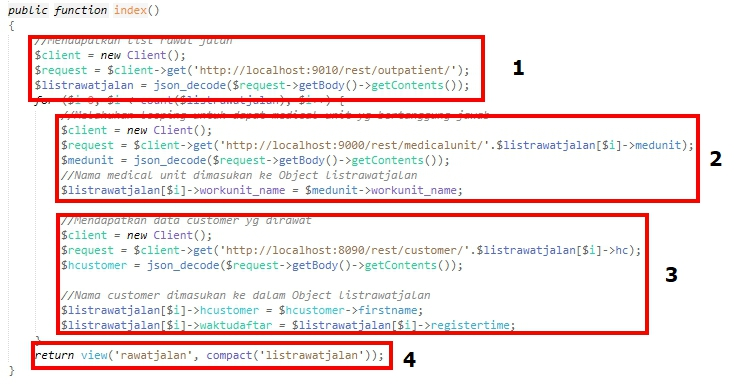
\includegraphics[width=12cm]{images/join.jpg}}	
			\captionof{figure}{\textit{In-memory join} untuk rawat jalan.}
		\end{minipage}
	\end{adjustbox}
	\end{table}
	\newpage
	\item Tingkat Availabilitas.
	\begin{table}[H]
		\small
		\begin{adjustbox}{width=1\textwidth}
			\begin{tabular}{| p {2 cm} | p {10 cm} |}
				\hline
				Arsitektur & Perbandingan Tingkat Availabilitas\\
				\hline
				\textbf{Monolitik} & Untuk membandingkan seberapa besar tingkat availabilitas dari sistem Apertura, maka akan diangkat sebuah skenario masalah yang pernah terjadi pada sistem, yaitu ketika sistem diharuskan untuk sementara waktu berada pada \textit{status down} untuk melakukan \textit{maintenance} atau perbahan pada \textit{database}. Dalam penelitian ini, modul-modul yang tercipta untuk jasa rawat jalan rumah sakit ada 4 modul, yaitu modul \textit{customer, human resources, medical unit,} dan modul \textit{outpatient}. Total fitur yang ada dari semua modul tersebut berjumlah 13 fitur.
				
				(\textit{Customer}: Menampilkan data pasien dan mencari pasien. \textit{Human Resources}: Menampilkan data dokter, edit data dokter, dan mencari dokter. \textit{Medical Unit}: Menampilkan data \textit{medical unit}, menambah \textit{medical unit} baru, menghapus \textit{medical unit}, dan mencari \textit{medical unit}. \textit{Outpatient}: Menampilkan, menambah, menghapus, dan mencari data rawat jalan.)
				
				Dalam arsitektur monolitik, \textit{status down} yang terjadi mengharuskan sistem untuk tidak berfungsi sementara, yang dimana berarti semua fitur tidak akan berfungsi seluruhnya dikarenakan modul-modul bergantung pada 1 buah database dalam sebuah \textit{server} terpusat.
				\\
				\hline
				\textbf{Microservice} & Pada model arsitektur microservice, \textit{status down} yang terjadi tidak akan menyebabkan keseluruhan fitur menjadi lumpuh. Misalnya apabila mengharuskan terjadi \textit{down} pada modul rawat jalan, maka fitur menampilkan, menambah, menghapus, dan mencari data rawat jalan akan tidak dapat berfungsi, namun 9 fitur yang lain seperti melihat unit medis bertugas, melihat data dokter dan data pasien akan tetap berjalan dengan normal. Menjadikan sistem lebih \textit{high availability}.
				
				\textit{Drawback} : 
				\begin{enumerate}[leftmargin=*]
					\item Cost yang lebih besar dikarenakan kebutuhan menyiapkan \textit{server} tambahan untuk setiap service yang di\textit{deploy}.
					\item Dibutuhkan usaha yang lebih besar untuk mengawasi banyak \textit{server}.
				\end{enumerate}\\
				\hline
			\end{tabular}
		\end{adjustbox}
	\end{table}
	\newpage
	\item Skalabilitas.
	\begin{table}[H]
		\small
		\begin{adjustbox}{width=1\textwidth}
			\begin{tabular}{| p {2 cm} | p {10 cm} |}
				\hline
				Arsitektur & Perbandingan Skalabilitas Sistem\\
				\hline
				\textbf{Monolitik} & Skenario yang dapat diangkat untuk melihat seberapa besar tingkat skalabilitas dari perangkat lunak Apertura adalah dengan menganalisa bagaimana sistem akan berubah saat sistem menjadi besar. Dalam arsitektur monolitik, sistem dapat direplikasi menjadi 2 buah monolitik yang identik. Kegunaan dari replikasi ini adalah mengantisipasi apabila sistem pertama tidak dapat atau mulai turun performanya ketika sistem bertambah besar, maka sistem replika siap membantu. Sebagai contoh sistem pertama mulai sibuk dengan pendaftaran antrian rawat jalan yang baru, maka sistem replika dapat membantu untuk menangani permintaan melihat unit medis bertugas atau melihat data dokter. Namun kelemahan dari metode ini pada monolitik adalah replikasi membutuhkan biaya yang besar dikarenakan sistem monolitik yang begitu besar dan tidak terpisahkan.\\
				\hline
				\textbf{Microservice} & Sifat microservice yang 'moduler' baik sebagai solusi untuk mendukung sistem ketika sistem butuh beradaptasi. Service yang cenderung sibuk dapat direplikasi dan diakses menggunakan alamat API yang berbeda dan disimpan pada databasenya masing-masing. Misalnya untuk kasus rawat jalan, pendaftaran dapat menggunakan 2 service rawat jalan yang berbeda halaman. Lalu data dari 2 service tersebut di \textit{load} dan ditampilan pada halaman rawat jalan kemudian \textit{sorting} berdasarkan waktu pendaftaran. Kelebihan yang dirasakan adalah replikasi tidak mengharuskan dilakukan pada keseluruhan sistem, melainkan hanya modul yang lebih padat.
				
				\textit{Drawback} : 
				\begin{enumerate}[leftmargin=*]
					\item Melakukan \textit{deployment} pada microservice lebih kompleks karena memungkinkan konfigurasi yang berbeda untuk setiap service.
					\item Membutuhkan integrasi lanjutan agar dapat bersinergi dengan service lain. Misalnya harus memberi tahu service lain apabila terjadi perubahan alamat IP (internet protocol) pada \textit{web API}.
				\end{enumerate}\\
				\hline
			\end{tabular}
		\end{adjustbox}
	\end{table}
\end{enumerate}
\newpage